%!TEX root = tcc_proposta.tex
\chapter{Trabalho Proposto}\label{chap3:proposal}

    Neste capítulo será apresentada a metodologia utilizada nesse trabalho, cujo objetivo é seguir um processo científico. Também apresentamos o detalhamento dos nossos objetivos e um cronograma com descrição das atividades a serem realizadas.

    \section{Metodologia}
       Este trabalho vem sendo realizado seguindo a seguinte metodologia: 
        
        \begin{enumerate}[label=\alph*)]
            \item Identificação de um Problema de Pesquisa: a partir da análise do trabalho de Jurak~\cite{JURAK2020} foi possível observar que evasão de colisão aplicado a USV é uma demanda atual, e que determinar se um encontro entre duas embarcações resultará em colisão é uma necessidade em sistemas para USV. Com isso, originou-se a pergunta de pesquisa que guiará este trabalho:
            
            \vspace{3mm}
            
            \centerline{\textit{"Como identificar situações de colisões no âmbito de USVs?"}}
            
            \item Definição da Sentença de Busca: a partir da pergunta formulada na etapa anterior, obteve-se o entendimento de quais áreas seriam permeadas para respondê-la. Com esse entendimento, extraiu-se as palavras chaves formulando a seguinte sentença de busca:
            
            \vspace{3mm}
            
            \centerline{\textit{"USV" AND "COLREGS" AND "collision avoidance"}}
            
            \item Seleção de Trabalhos Relacionados: aplicando a sentença de busca definida em bases de busca como IEEE Explorer\footnote{https://ieeexplore.ieee.org/Xplore/home.jsp}, Scopus\footnote{https://www.scopus.com/search/form.uri?display=basic} e Science Direct\footnote{https://www.sciencedirect.com/}, foi realizada a pré-seleção de trabalhos que poderiam embasar o trabalho proposto. A pré-seleção foi feita com base na leitura do \textit{"abstract"} do trabalho e da dissertação acerca de evasão de colisão e CPA, resultando em 28 trabalhos pré-selecionados. Posteriormente, através de uma análise mais detalhada dos trabalhos, para identificar as técnicas utilizadas, e considerando seus respectivos Índice H, foram selecionados os 5 trabalhos mais relevantes para serem utilizados como referência neste trabalho.
            
            \item Leitura dos Trabalhos Selecionados e Extração de Conhecimentos Relevantes: para obter um conhecimento mais aprofundado a respeito da área, do problema e das técnicas utilizadas pelos autores atualmente, foi realizada a leitura completa dos trabalhos atentando para a fundamentação teórica e analisando brevemente seus resultados. Com isso foi possível compreender como implementar CPA e quais resultados esperar da implementação.
            
            \item Estruturar a Proposta de Trabalho: com o conhecimento obtido da etapa anterior foi possível estruturar a presente proposta de trabalho contendo uma contextualização, embasamento teórico, objetivos e os meios que serão utilizados para atingi-los.
            
            \item Implementação da Proposta Aceita: com a proposta analisada e aprovada pelos avaliadores, será realizada a implementação do CPA e a integração com o sistema desenvolvido por Jurak~\cite{JURAK2020}, seguindo o cronograma apresentado na Figura~\ref{fig:chap3_schedule}.
            
            \item Executar Casos de Testes: validar a implementação realizada a partir de casos específicos de testes, a fim de estressar a implementação e obter possíveis comportamentos não previstos durante a implementação do sistema.
            
            \item Análise dos Resultados: analisar o comportamento obtido na fase de testes e compará-lo com o comportamento anterior à implementação deste trabalho. Também será realizada uma comparação com os resultados obtidos pelos demais autores da área. 
        \end{enumerate}
        
    \section{Objetivos}
    
        O principal objetivo deste trabalho é implementar uma aplicação capaz de calcular o CPA de um encontro entre embarcações e, quando em situação de colisão, gerar o VO do encontro. Devido ao curto tempo de implementação, o algoritmo VO não será utilizado para resolver uma situação de colisão (como apresentado por Kuwata~\etal~\cite{KUWATA2014110}, Huang~\etal~\cite{HUANG2019142} e Song~\etal~\cite{SONG2018351}), mas adaptaremos a solução para, quando em situação de colisão, gerar obstáculos virtuais adicionais no sistema de Jurak~\cite{JURAK2020}. Estes obstáculos serão gerados utilizando o mesmo padrão apresentado por Jurak~\cite{JURAK2020} em seu trabalho e ocuparão a área resultante do algoritmo VO. Como resultado, após integração da aplicação desenvolvida neste trabalho no sistema de Jurak~\cite{JURAK2020}, é esperado que o sistema identifique encontros em que ocorrerá colisão e, principalmente, encontros que não ocorrerá colisão. Quando em situação de colisão, é esperado que o algoritmo VO seja acionado e os obstáculos virtuais adicionais acreça segurança ao sistema.
        
        Como objetivo secundário, realizaremos a integração completa da aplicação desenvolvida neste trabalho no sistema de Jurak~\cite{JURAK2020}. Serão simulados testes em diferentes encontros através do simulador USV\_sim\footnote{\url{https://github.com/disaster-robotics-proalertas/usv\_sim\_lsa}}~\cite{Paravisi2018Toward} com a finalidade de estressar a solução e garantir que o objetivo principal foi atingido. Por fim, realizar-se-a um comparativo entre os resultados obtidos com o novo comportamento do sistema e os resultados anteriores à implementação deste trabalho, além de comparações com resultados obtidos pelos autores da literatura de referência.
        
    \section{Cronograma}
        A Figura~\ref{fig:chap3_schedule} apresenta detalhadamente o cronograma de atividades, previstas e já realizadas, para atingir os objetivos expostos nesse documento. O planejamento foi realizado considerando atividades por semana e prevê, de forma geral, as seguintes atividades:\frm{Muito genérico. Tua tabela abaixo está melhor detalhada, use ela como base.}
        \begin{enumerate}
            \item \textbf{Escrita}: elaboração dos arquivos contendo a informações necessárias para a documentação do processo de desenvolvimento do trabalho. Nessa atividade serão gerados dois documentos: a proposta de trabalho e o volume final.
            
            \item \textbf{Estudo da Literatura}: pesquisa realizada para adquirir conhecimento básico a respeito do tema, como a respeito de USV e COLREGS, além de realizar um estudo aprofundado das técnicas utilizadas hoje em dia para detectar CPA e gerar um VO.
            
            \item \textbf{Estudo do Framework de Desenvolvimento}: prática a ser realizada com as ferramentas necessárias para o desenvolvimento do trabalho proposto.
            
            \item \textbf{Implementação}: tempo previsto para a codificação do CPA e do VO.
            
            \item \textbf{Coleta e Análise dos Resultados}: realização de testes com a finalidade de validar e avaliar o resultado final. Esses resultados serão comparados com os obtidos por Jurak~\cite{JURAK2020}, em seu trabalho original, bem como com os resultados de outros autores que também utilizaram da mesma técnica.
        \end{enumerate}
        
        \begin{figure}[htb]
            \centering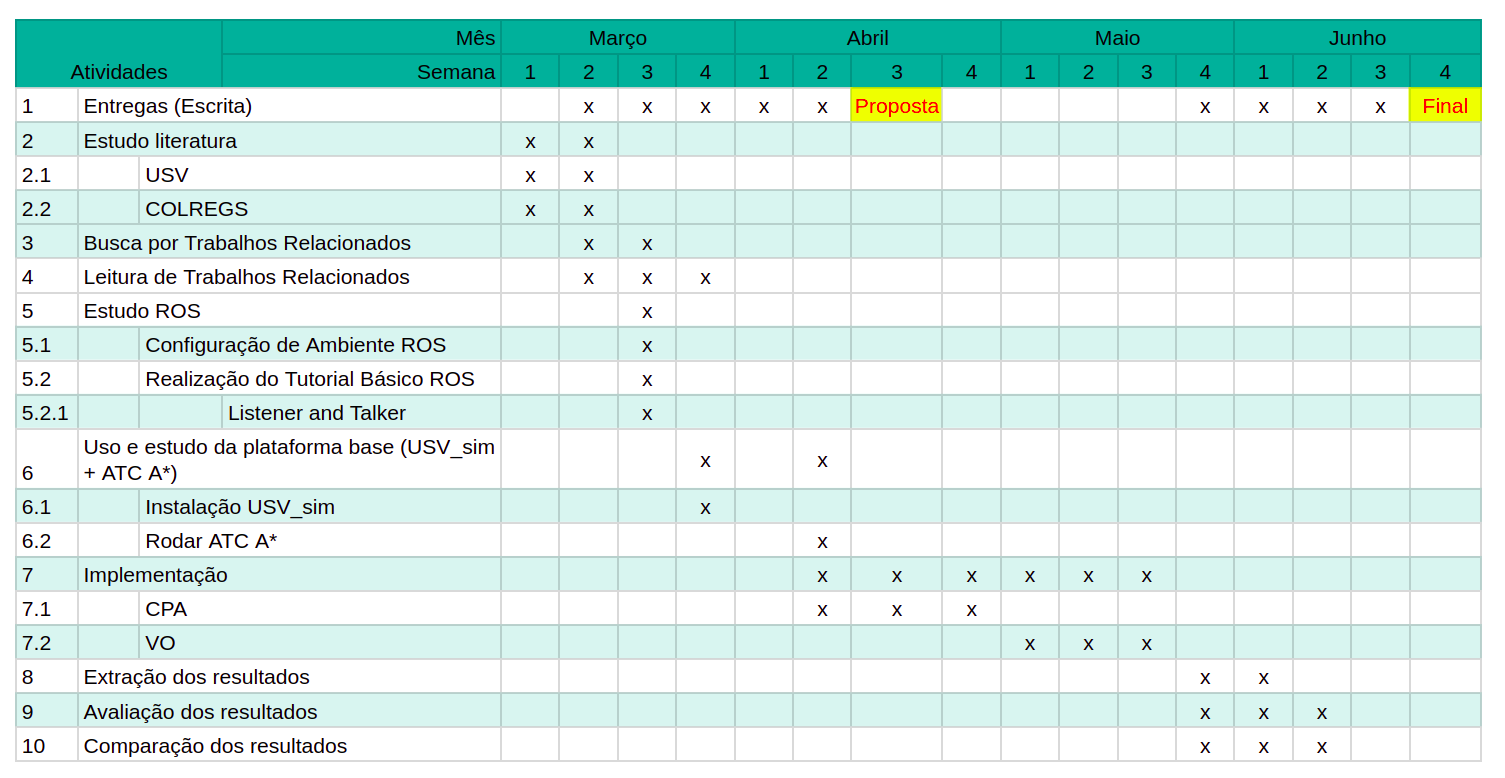
\includegraphics[width=1.3\textwidth, angle=90]{fig/chap3/schedule.png}
            \caption{\label{fig:chap3_schedule} Cronograma proposto para realização das atividades.}
        \end{figure}